\title{Final Exam for Calculus-Based Physics-2: Electricity, Magnetism, and Thermodynamics (PHYS180-02)}
\author{Dr. Jordan Hanson - Whittier College Dept. of Physics and Astronomy}
\date{\today}
\documentclass[10pt]{article}
\usepackage[a4paper, total={18cm, 27cm}]{geometry}
\usepackage{outlines}
\usepackage[sfdefault]{FiraSans}
\usepackage{hyperref}
\usepackage{graphicx}
\begin{document}
\maketitle

\begin{enumerate}
\item \textbf{Temperature and Heat}
\begin{enumerate}
\item A metal beam is manufactured slightly longer than the specifications, at a location which is on average 30 degrees C colder than the construction site.  Which of the following is true?
\begin{itemize}
\item A: The beam will fit into the design because it will change in length.
\item B: The beam will fit into the design because it will not change in length.
\item C: The beam will not fit into the design because it will change in length.
\item D: The beam will not fit into the design because it will not change in length.
\end{itemize}
\item Recall that the linear expansion of materials is described by $\Delta L = \alpha L_0 \left(T_f - T_i \right)$.  The linear expansion coefficient of steel is $12 \times 10^{-6}$ C$^{\circ -1}$.  If a steel beam is 10.0 m long at 0 C$^{\circ}$, what is the change in length if the beam temperature is raised by 40 C$^{\circ}$?  Graph the length of the beam versus temperature, and indicate the length at 0 and 40 C$^{\circ}$.  \\ \vspace{3cm}
\end{enumerate}
\item \textbf{The Kinetic Theory of Gases}
\\ \\ Recall that $pV = n R T$, and that $\Delta E_{int} = \frac{3}{2} n R \Delta T$ for a monatomic ideal gas.
\begin{enumerate}
\item An ideal gas is held at constant temperature.  The volume is 2.0 L.  If the pressure doubles, what is the new volume?  \\ \vspace{1cm}
\item An ideal gas is held at constant temperature and volume.  There are 3.0 moles of the gas.  If the pressure doubles, what is the new number of moles?  \\ \vspace{1cm}
\item Suppose a small piston contains 1.0 mole of an ideal gas, at a pressure of 2 atm in a volume of 2 L.  What is the temperature?
\begin{itemize}
\item A: 50 Kelvin
\item B: 20 Kelvin
\item C: 10 Kelvin
\item D: 100 Kelvin
\end{itemize}
\item Same piston as the previous question.  If heat is added such that the piston expands to 4 L \textbf{\textit{isothermically}}, what is the new pressure?
\begin{itemize}
\item A: 4 atm
\item B: 3 atm
\item C: 2 atm
\item D: 1 atm
\end{itemize}
\item What is the change in internal energy of the cylindar system from the previous question? \\ \vspace{1cm}
\item Recall that $Q = n C_V \Delta T$, and that for an ideal monatomic gas, $C_V = \frac{d}{2}R$, where $d$ is the number of degrees of freedom.  How much heat is required to raise the temperature of 2.0 moles of a diatomic ideal gas by $10$ C$^{\circ}$, if (a) we account for just translational motion and (b) if we account for translational and rotational motion? \\ \vspace{2cm}
\end{enumerate}
\item \textbf{The First Law of Thermodynamics}
\\ \\ Recall that $\Delta E_{int} = Q - W$, and that $dW = p dV$ at constant pressure.
\begin{enumerate}
\begin{figure}
\centering
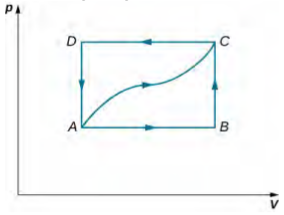
\includegraphics[width=0.25\textwidth]{figures/pvdiag.png}
\caption{\label{fig:pvdiag} A pV diagram illustrating thermodynamic processes.}
\end{figure}
\item Observe Fig. \ref{fig:pvdiag}.  Which process does the most net work?
\begin{itemize}
\item A: ABCDA
\item B: ACDA
\item C: ABCA
\item D: ADCBA
\end{itemize}
\item Let state D be (4 L, 4 atm), state C be (8 L, 4 atm), state B be (8 L, 2 atm), and state A be (4 L, 2 atm).  What is the net work of process DCBAD?
\begin{itemize}
\item A: 4 L atm
\item B: 8 L atm
\item C: 2 L atm
\item D: 1 L atm
\end{itemize}
\item If the change in internal energy of a system is 100 J, and the system does 250 J of work, how much heat was added? \\ \vspace{2cm}
\end{enumerate}
\item \textbf{The Second Law of Thermodynamics}
\\ \\ Recall that $e = 1-\frac{T_c}{T_h}$, and that $W = e Q_h$.
\begin{enumerate}
\item What amount of work is done by a Carnot engine that has a high temperature of 900 K and a low temperature of 300 K, if the heat injected is 1 kJ? \\ \vspace{3cm}
\end{enumerate}
\item \textbf{Electric Charges and Fields}
\begin{enumerate}
\item Recall that $\vec{E} = k \frac{q_1}{r^2}\hat{r}$.  (a) Eight charges are all on the x-axis, with equal distances between them.  At what locations, if any, is the electric field equal to zero?  (b) Seven charges are all on the x-axis, with equal distances between them.  At what locations, if any, is the electric field equal to zero? \\ \vspace{2cm}
\item (a) Draw the electric field of an electric dipole (two charges separated by some distance and of opposite magnitude). (b) Draw the electric field of two dipoles that are next to each other, but pointing in the opposite direction (a square of charge with two positives and two negatives).  This is known as a quadrupole.  \\ \vspace{3cm}
\item Which of the following is true of an infinite plane of positive charge in the x-y plane?
\begin{itemize}
\item A: The field increases with increasing $z$.
\item B: The field decreases with increasing $x$ or $y$.
\item C: The field does not depend on $x$ or $y$.
\item D: The field has a $\hat{z}$ component.
\item E: C and D
\end{itemize}
\end{enumerate}
\item \textbf{Gauss's Law}
\begin{enumerate}
\item Suppose an infinite line of charge is oriented along the $z$ axis, and the charge per unit length area is $\lambda$.  Using Gauss' Law, derive the electric field (\textit{use a cylinder as the Gaussian surface}). \\ \vspace{2.5cm}
\end{enumerate}
\item \textbf{Electric Potential}
\\ \\ Recall that $\vec{E} = -\vec{\nabla} V(x,y,z)$, and that $V = E z$ for a uniform E-field.
\begin{enumerate}
\item What is the electric field associated with the voltage $V(x,y,z) = V_0 \left( 2x + xy^3 \right)$?  Remember to express your answer as a \textit{vector field}, not just a magnitude of a field.  \\ \vspace{1.5cm}
\item Suppose two charged plates create a uniform electric field between them.  If the field is 1 kV/m, and the separation between the plates is 1 cm, what is the voltage between the plates?  \\ \vspace{1.5cm}
\item What energy would be gained by a proton if released through the voltage in the previous problem? \\ \vspace{1.5cm}
\end{enumerate}
\item \textbf{Current and Resistance}
\begin{enumerate}
\item Recall that $V = iR$, and that $R = \frac{\rho L}{A}$.  Suppose current is flowing through a cylindrical wire with radius $r$ and length $l$.  The voltage driving the current remains constant.  \textbf{\textit{Choose all that are true}}:
\begin{itemize}
\item A: If the current is 10 A when the $l=10$ meters, the current will be 20 A when the $l=20$ meters.
\item B: If the current is 10 A when the $l=10$ meters, the current will be 5 A when the $l=20$ meters.
\item C: If the current is 10 A when the $r=2$ mm, the current will be 5 A when the $r=1$ mm.
\item D: If the current is 10 A when the $r=2$ mm, the current will be 2.5 A when the $r=1$ mm.
\end{itemize}
\begin{figure}[hb]
\centering
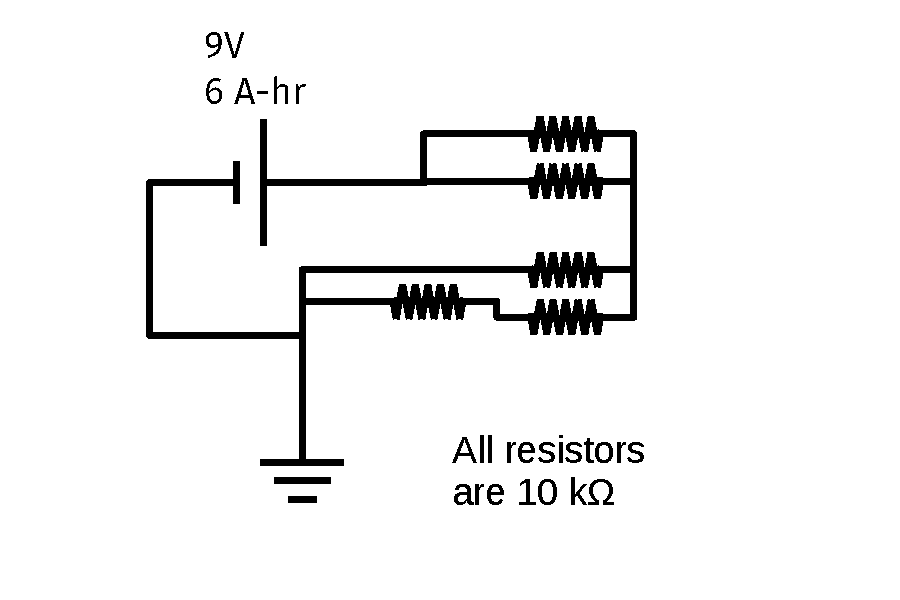
\includegraphics[width=0.5\textwidth]{figures/circuitExample2.pdf}
\caption{\label{fig:circuit} A DC circuit with a battery voltage of 9V and identical resistors.}
\end{figure}
\item Consider the circuit in Fig. \ref{fig:circuit}.  How long before the battery runs out? \\ \vspace{3cm}
\end{enumerate}
\item \textbf{Magnetic Forces and Fields}
\begin{figure}
\centering
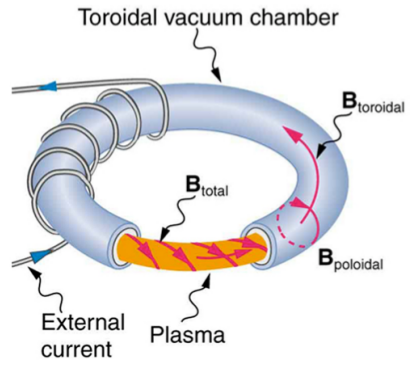
\includegraphics[width=0.3\textwidth]{figures/tok.png}
\caption{\label{fig:tok} The basic premise of a tokamak, containing plasma for fusion reactions.}
\end{figure}
\\ \\
\textit{Recall that $\vec{F} = q\vec{v} \times \vec{B}$.} The toroidal magnetic field in the tokamak fusion reactor in Fig. \ref{fig:tok} is created by the external current.  The plasma is hot ionized gas, and the \textit{poloidal} magnetic field is created by it.
\begin{enumerate}
\item Suppose the current is reversed in Fig. \ref{fig:tok}.  What will be the direction of the toroidal magnetic field and poloidal magnetic field at the bottom of the ring where it says ``plasma''?
\begin{itemize}
\item A: Right, up
\item B: Left, up
\item C: Left, down
\item D: Right, down
\end{itemize}
\end{enumerate}
\end{enumerate}
\end{document}